\documentclass[a4paper,11pt]{article}
\usepackage[utf8]{inputenc}
\usepackage[T1]{fontenc}
\usepackage[french]{babel}
\usepackage{makeidx}
\usepackage{textcomp}
\usepackage{graphicx}
\usepackage{mathtools,amssymb,amsthm}
\usepackage{lmodern}
\usepackage{multirow}
\usepackage{array}
\usepackage{longtable}

\title{TER 2019 - Spécifications}
\author{Maxime Gonthier - Benjamin Guillot - Laureline Martin}
\begin{document}
	\pagenumbering{gobble}\clearpage
	\maketitle

\newpage
\tableofcontents

\newpage
\section{Modélisation des données}
	On va répartir les données concernant la fac en 4 modules.\\
	(Preciser ce qu'est un module)
	\begin{itemize}
		\item Module cours
		\item Module salle de classe
		\item Module étudiant
		\item Module professeur
	\end{itemize}
	\subsection{Module Cours}
		Le module cours est une classe représentant un cours sur un temps donné.\\
		Lors des affectations, on modifiera pour chaque instance a deplacer l'horaire de début.\\
		Elle contient : 
		\begin{enumerate}
			\item duree : un entier -représente la durée du cours en minutes-
			\item liste_etu : un tableau d'entier qui contient les numero des étudiants participant à ce cours.
			\item type_salle : un entier, 0 pour une salle de TP et 1 pour un autre salle (on pourra ajouter d'autres type de salle si necessaire).
			\item num_salle : un entier (identifiant unique représentant la salle)
			\item num_ens : un entier désignant le professeur donnant ce cours(identifiant unique représentant le professeur)
			\item debut : un entier pour l'heure, un entier pour la minute (structure implémentée specialement pour le projet)  
			\item fin : un entier pour l'heure, un entier pour la minute.
			\item liste_ens : une liste contenant les identifiants des professeurs pouvant enseigner ce cours.
		\end{enumerate}
	\subsection{Module Salle de classe}
		Le module salle représente la localisation du cours sur un temps donné.
		\begin{enumerate}
			\item num_salle : un entier (identifiant unique)
			\item localisation : un entier -0 pour proche de l'arrêt de bus desservant l'université, 1 pour modérément éloigné, 2 pour éloigné-. 
			\item type_salle : un entier, 0 pour une salle de TP et 1 pour une autre salle (on pourra ajouter d'autres type de salle si necessaire).
			\item capacite : un entier désigant le nombre maximal d'étudiant que peut contenir la salle
		\end{enumerate}
	\subsection{Module Etudiant}
		Le module étudiant représente un élève, il sera représenté par :
		\begin{enumerate}
			\item distance : un entier qui représente la distance entre le domicile de l'étuidant et l'université, 0 si l'étudiant habite a moins de 15 min de la fac, 1 si il habite entre 15 et 45 min de la fac, 2 sinon.
			\end{enumerate}
	\subsection{Module Professeur}
		\begin{enumerate}
			\item num_ens : un entier (identifiant unique)
			\item plage : un tableau dont chaque case représente un bloc horaire (15 min par exemple)
			Si xi vaut 0 alors c'est l'horaire du début de la disponibilité, si xi vaut 1 c'est la fin de la disponibilité du professeur.
			\end{enumerate}
	\subsection{Matrice d'adjacence entre les salles}
		Cette matrice va indiquer la distance entre deux salles. Elle est symétrique. Si la distance prend moins de 15 min à parcourir a pied on met 0.
		Entre 15 et 30 min on met 1. Plus de 30 min on met 2.
	\subsection{Matrice d'adjacence entre salles et arrêt de bus}
		De même mais cette fois la matrice a une seule colonne représentant l'arrêt de bus desservant l'université.
		On regarde alors le temps que l'ont met pour aller de l'arrêt de bus a la salle et on remplit de la même manière que pour la matrice précédente.
	\subsection{Conclusion des liens entre les modules}
		\centerline{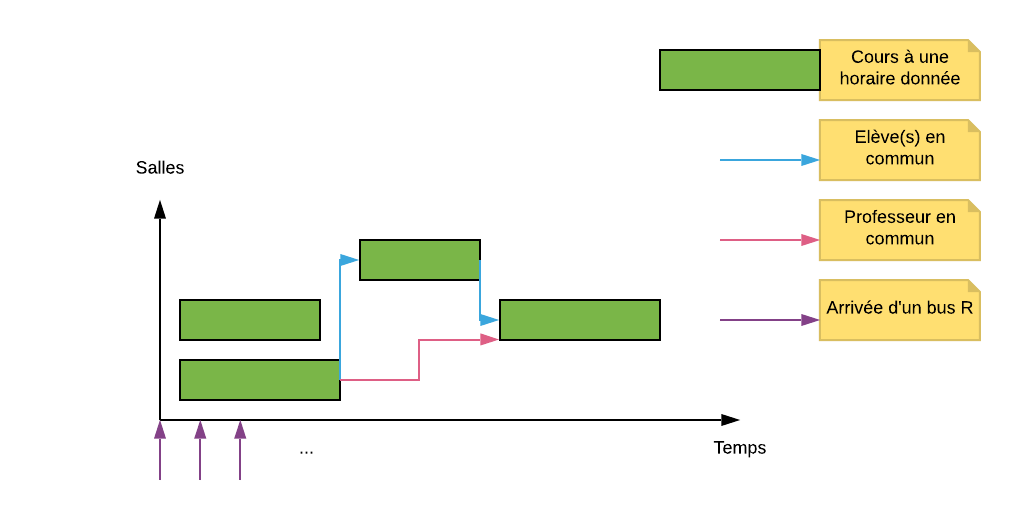
\includegraphics[scale=0.5]{modelter.png}}
		Modélisation.\\
	

\section{Les fonctions principales}
	\subsection{Calcul indice de flexibilité}
		Cette fonction prendra en entrée la flexibilité de chaque étudiant assistant à un cours donné et en fera la somme. 
		Un indice de flexibilité est ainsi calculé, cette modelisation a pour but de favoriser les cours ayant le plus d'etudiants.\\
		
	\subsection{Calcul flexibilité étudiant}
		Cette fonction prend en entrée la distance entre le domicile de l'étudiant et l'université ainsi que les contraintes
		associées à l'étudiant (si il en possède). La fonction calcule et renvoie la flexibilité de l'étudiant.
	\subsection{Y a forcément d'autres fonctions}

\section{Contraintes}
	Pour optimiser, nous faisons face à plusieurs contraintes, toutes ne sont pas 
	de même "importances". Nous allons donc devoir définir un ordre de priorité sur 
	les contraintes, ainsi lors de l'optimisation par notre algorithme, nous 
	pourrons ajuster et obtenir de meilleurs résultats même si certaines contraintes
	"faibles" sont violées.\\
	\subsection{Contraintes dures}
		\begin{enumerate}
			\item 0 : Entre deux cours : Si deux cours utilisent la même salle à des horaires qui se chevauchent ou
			si il y a des élèves en commun sur deux cours dont les horaires se chevauchent.
			\item 1 : Entre un cours et un professeur : Le professeur doit pouvoir enseigner ce cours. D'où la création de la liste de professeur pouvant enseigner un cours dans le module cours.
			On regarde aussi si la plage de disponibilité du professeur correspond à l'horaire du cours.
			\item 2 : Entre un cours et une salle : La salle doit avoir une capacité supérieure ou égale au nombre d'élèves suivant le cours et doit correspondre au type de salle dont le cours a besoin.
			On ne précise pas la contraintes entre cours et étuidant car un étudiant est défini par ses cours.
		\end{enumerate}
	\subsection{Contraintes faibles}
		\begin{enumerate}
			\item 3 : Avoir une personne à charge ce qui impose un horaire le matin et/ou le soir.
			Exemple : Sois X l'heure de début d'un cours, si un enfant doit être déposé à l'école à 9h on a : X > 9 + (indice de distance de cet étudiant)*30 min
			Sois Y l'heure de fin d'un cours, si un enfant doit être récupéré à l'école à 17h on a : Y < 17 - (indice de distance de cet étudiant)*30 min
			\item 4 : Avoir un travail, cela impose la même chose que la contraintes précédentes
		\end{enumerate}

	\subsection{Module Contraintes}  
		\begin{itemize}
			\item identifiant : un entier non unique correspondant à une des contrainte precedement. L'identifiant représente une hierarchie dans les contraintes, de la plus forte a la plus faible 
			\item un tableau d'entier contenant les identifiant des étudiants sujet à cette contrainte.
	%\subsection{Sélections par heuristiques}
		%Les différentes heuristiques que nous allons utiliser pour jouer sur les 
		%contraintes. $$surement tabou$$ \\
		\end{itemize}
\section{Affectation}
	On va affecter chaque cours à un horaires sans prendre en compte les transports. On ne va utiliser que les contraintes énoncés précédemment. \\
	A chaque cours on affecte une horaire de début (l'horaire de fin est calculé en conséquence), tel que les contraintes dures sont validées.
	On va utiliser une heuristique tabou. On commence avec un emploi du temps par défaut. Le voisinage correspond à la modification d'un cours. A chaque itération on recalcule le nombre de contraintes violées. Un optimum local sera une solution viable, c'est à dire qui ne viole pas les contraintes dures.
	(Si les solutions trouvées boucle (c'est à dire si les résultats restent similaires) alors on va éloigner le voisnage A REDIRE MIEUX)
	(Relier l'affectation aux bus)
	
\section{Implémentation des bus}
	Pour les transports, on supposera que chaque élève arrivera par le bus précédant le début du premier cours de sa journée. De cette manière a chaque itération de l'affectation des cours, on pourra recalculer la congestion de chaque bus (qui sera utilisé comme fonction objectif du projet une fois les transport implémentés).La congestion peut être représentée par le pourcentage de remplissage du bus à chaque arrêt. 

\section{Métrique d'évaluation}
	(congestion + contraites faibles)

\end{document}
